\documentclass[border=0.1cm]{standalone}
\usepackage{tikz}
\usepackage{amsfonts}
\usepackage{amsmath,amssymb}
\usepackage{systeme,mathtools}
\usetikzlibrary{positioning,arrows.meta,quotes}
\usetikzlibrary{shapes,snakes}
\usetikzlibrary{bayesnet}
\tikzset{>=latex}
\tikzstyle{plate caption} = [caption, node distance=0, inner sep=0pt,
below left=5pt and 0pt of #1.south]
\begin{document}
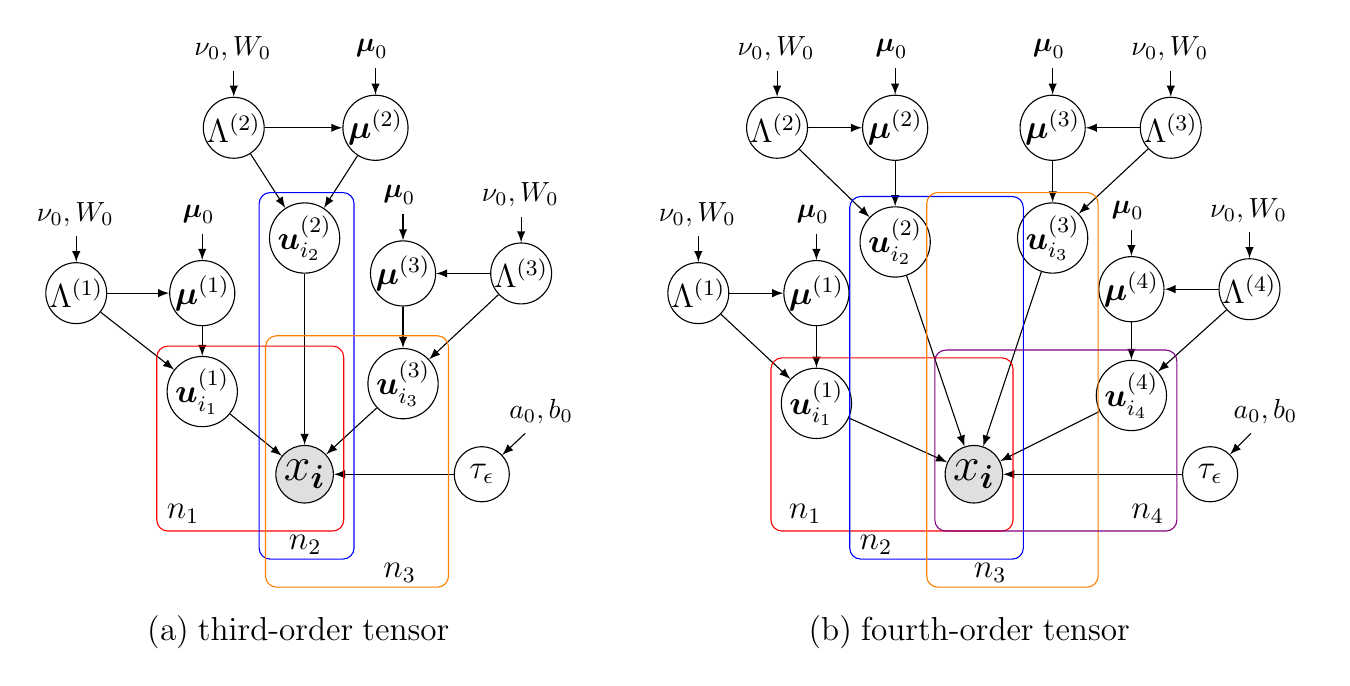
\begin{tikzpicture}
	% Third-order tensor
    \node [obs] (x) at (2,1) {\LARGE $x_{\boldsymbol{i}}$};
    \node [circle,draw=black,fill=white,inner sep=0pt,minimum size=0.5cm] (u1) at (0.7,2.05) {\large $\boldsymbol{u}_{i_1}^{(1)}$};
    \node [circle,draw=black,fill=white,inner sep=0pt,minimum size=0.5cm] (u2) at (2,4) {\large $\boldsymbol{u}_{i_2}^{(2)}$};
    \node [circle,draw=black,fill=white,inner sep=0pt,minimum size=0.5cm] (u3) at (3.25,2.15) {\large $\boldsymbol{u}_{i_3}^{(3)}$};
    \node [circle,draw=black,fill=white,inner sep=0pt,minimum size=0.5cm] (mu1) at (0.7,3.3) {\large $\boldsymbol{\mu}^{(1)}$};
    \node [circle,draw=black,fill=white,inner sep=0pt,minimum size=0.5cm] (lambda1) at (-0.9,3.3) {\large $\Lambda^{(1)}$};
    \node [circle,draw=black,fill=white,inner sep=0pt,minimum size=0.5cm] (mu2) at (2.9,5.4) {\large $\boldsymbol{\mu}^{(2)}$};
    \node [circle,draw=black,fill=white,inner sep=0pt,minimum size=0.5cm] (lambda2) at (1.1,5.4) {\large $\Lambda^{(2)}$};
    \node [circle,draw=black,fill=white,inner sep=0pt,minimum size=0.5cm] (mu3) at (3.25,3.55) {\large $\boldsymbol{\mu}^{(3)}$};
    \node [circle,draw=black,fill=white,inner sep=0pt,minimum size=0.5cm] (lambda3) at (4.75,3.55) {\large $\Lambda^{(3)}$};
    \node [text width=0.5cm] (mu01) at (0.7,4.30) {$\boldsymbol{\mu}_0$};
    \node [text width=1cm] (nuW1) at (-0.9,4.30) {$\nu_0,W_0$};
    \node [text width=0.5cm] (mu02) at (2.9,6.4) {$\boldsymbol{\mu}_0$};
    \node [text width=1cm] (nuW2) at (1.1,6.4) {$\nu_0,W_0$};
    \node [text width=0.5cm] (mu03) at (3.25,4.55) {$\boldsymbol{\mu}_0$};
    \node [text width=1cm] (nuW3) at (4.75,4.55) {$\nu_0,W_0$};
    
    \node [circle,draw=black,fill=white,inner sep=0pt,minimum size=0.7cm] (tau_epsilon) at (4.25,1) {\large $\tau_{\epsilon}$};
    \node [text width=1cm] (ab0) at (5.1,1.8) {$a_0,b_0$};
    
    \path [draw,->] (u1) edge (x);
    \path [draw,->] (u2) edge (x);
    \path [draw,->] (u3) edge (x);
    \path [draw,->] (mu1) edge (u1);
    \path [draw,->] (lambda1) edge (u1);
    \path [draw,->] (lambda1) edge (mu1);
    \path [draw,->] (mu2) edge (u2);
    \path [draw,->] (lambda2) edge (u2);
    \path [draw,->] (lambda2) edge (mu2);
    \path [draw,->] (mu3) edge (u3);
    \path [draw,->] (lambda3) edge (u3);
    \path [draw,->] (lambda3) edge (mu3);
    \path [draw,->] (mu01) edge (mu1);
    \path [draw,->] (nuW1) edge (lambda1);
    \path [draw,->] (mu02) edge (mu2);
    \path [draw,->] (nuW2) edge (lambda2);
    \path [draw,->] (mu03) edge (mu3);
    \path [draw,->] (nuW3) edge (lambda3);
    
    \path [draw,->] (tau_epsilon) edge (x);
    \path [draw,->] (ab0) edge (tau_epsilon);
    
    \plate [color=red] {part1} {(x)(u1)} { };
    \plate [color=blue] {part2} {(x)(u2)(part1.south east)} { };
    \plate [color=orange] {part3} {(x)(u3)(part2.south)(part1.north east)} { };
    \node [text width=2cm] at (1.25,0.5) {\large $n_1$};
    \node [text width=2cm] at (2.8,0.1) {\large $n_2$};
    \node [text width=2cm] at (4,-0.25) {\large $n_3$};
    \node [text width=4cm] at (2,-1) {\large (a) third-order tensor};
    
    % Fourth-order tensor
    \node [obs] (x_4) at (12-1.5,1) {\LARGE $x_{\boldsymbol{i}}$};
    \node [circle,draw=black,fill=white,inner sep=0pt,minimum size=0.5cm] (u1_4) at (10-1.5,1.9) {\large $\boldsymbol{u}_{i_1}^{(1)}$};
    \node [circle,draw=black,fill=white,inner sep=0pt,minimum size=0.5cm] (u4_4) at (14-1.5,2) {\large $\boldsymbol{u}_{i_4}^{(4)}$};
    \node [circle,draw=black,fill=white,inner sep=0pt,minimum size=0.5cm] (u2_4) at (11-1.5,3.95) {\large $\boldsymbol{u}_{i_2}^{(2)}$};
    \node [circle,draw=black,fill=white,inner sep=0pt,minimum size=0.5cm] (u3_4) at (13-1.5,4) {\large $\boldsymbol{u}_{i_3}^{(3)}$};
    \node [circle,draw=black,fill=white,inner sep=0pt,minimum size=0.5cm] (mu1_4) at (10-1.5,3.3) {\large $\boldsymbol{\mu}^{(1)}$};
    \node [circle,draw=black,fill=white,inner sep=0pt,minimum size=0.5cm] (lambda1_4) at (8.5-1.5,3.3) {\large $\Lambda^{(1)}$};
    \node [circle,draw=black,fill=white,inner sep=0pt,minimum size=0.5cm] (mu2_4) at (11-1.5,5.4) {\large $\boldsymbol{\mu}^{(2)}$};
    \node [circle,draw=black,fill=white,inner sep=0pt,minimum size=0.5cm] (lambda2_4) at (9.5-1.5,5.4) {\large $\Lambda^{(2)}$};
    \node [circle,draw=black,fill=white,inner sep=0pt,minimum size=0.5cm] (mu3_4) at (13-1.5,5.4) {\large $\boldsymbol{\mu}^{(3)}$};
    \node [circle,draw=black,fill=white,inner sep=0pt,minimum size=0.5cm] (lambda3_4) at (14.50-1.5,5.4) {\large $\Lambda^{(3)}$};
    \node [circle,draw=black,fill=white,inner sep=0pt,minimum size=0.5cm] (mu4_4) at (14-1.5,3.35) {\large $\boldsymbol{\mu}^{(4)}$};
    \node [circle,draw=black,fill=white,inner sep=0pt,minimum size=0.5cm] (lambda4_4) at (15.5-1.5,3.35) {\large $\Lambda^{(4)}$};
    \node [text width=0.5cm] (mu01_4) at (10-1.5,4.3) {$\boldsymbol{\mu}_0$};
    \node [text width=1cm] (nuW1_4) at (8.5-1.5,4.3) {$\nu_0,W_0$};
	\node [text width=0.5cm] (mu02_4) at (11-1.5,6.4) {$\boldsymbol{\mu}_0$};
	\node [text width=1cm] (nuW2_4) at (9.5-1.5,6.4) {$\nu_0,W_0$};
	\node [text width=0.5cm] (mu03_4) at (13-1.5,6.4) {$\boldsymbol{\mu}_0$};
    \node [text width=1cm] (nuW3_4) at (14.50-1.5,6.4) {$\nu_0,W_0$};
    \node [text width=0.5cm] (mu04_4) at (14-1.5,4.35) {$\boldsymbol{\mu}_0$};
    \node [text width=1cm] (nuW4_4) at (15.5-1.5,4.35) {$\nu_0,W_0$};
    \node [circle,draw=black,fill=white,inner sep=0pt,minimum size=0.7cm] (tau_epsilon4) at (15-1.5,1) {\large $\tau_{\epsilon}$};
    \node [text width=1cm] (ab0_4) at (15.8-1.5,1.8) {$a_0,b_0$};
    
    \path [draw,->] (u1_4) edge (x_4);
    \path [draw,->] (u2_4) edge (x_4);
    \path [draw,->] (u3_4) edge (x_4);
    \path [draw,->] (u4_4) edge (x_4);
    \path [draw,->] (mu1_4) edge (u1_4);
    \path [draw,->] (mu2_4) edge (u2_4);
    \path [draw,->] (mu3_4) edge (u3_4);
    \path [draw,->] (mu4_4) edge (u4_4);
    \path [draw,->] (lambda1_4) edge (mu1_4);
    \path [draw,->] (lambda1_4) edge (u1_4);
    \path [draw,->] (lambda2_4) edge (mu2_4);
    \path [draw,->] (lambda2_4) edge (u2_4);
    \path [draw,->] (lambda3_4) edge (mu3_4);
    \path [draw,->] (lambda3_4) edge (u3_4);
    \path [draw,->] (lambda4_4) edge (mu4_4);
    \path [draw,->] (lambda4_4) edge (u4_4);
    \path [draw,->] (mu01_4) edge (mu1_4);
    \path [draw,->] (nuW1_4) edge (lambda1_4);
    \path [draw,->] (mu02_4) edge (mu2_4);
    \path [draw,->] (nuW2_4) edge (lambda2_4);
    \path [draw,->] (mu03_4) edge (mu3_4);
    \path [draw,->] (nuW3_4) edge (lambda3_4);
    \path [draw,->] (mu04_4) edge (mu4_4);
    \path [draw,->] (nuW4_4) edge (lambda4_4);
    \path [draw,->] (tau_epsilon4) edge (x_4);
    \path [draw,->] (ab0_4) edge (tau_epsilon4);
    
    \plate [color=red] {part1} {(x_4)(u1_4)} { };
    \plate [color=blue] {part2} {(x_4)(u2_4)(part1.south east)} { };
    \plate [color=orange] {part3} {(x_4)(u3_4)(part2.south)(part1.south east)(part2.east)} {$ $};
    \plate [color=violet] {part4} {(x_4)(u4_4)(part2.east)(part3.east)} { };
    \node [text width=4.2cm] at (12-1.5,-1) {\large (b) fourth-order tensor};
    \node [text width=2cm] at (10.65-1.5,0.5) {\large $n_1$};
    \node [text width=2cm] at (11.55-1.5,0.1) {\large $n_2$};
    \node [text width=2cm] at (13-1.5,-0.25) {\large $n_3$};
    \node [text width=2cm] at (15-1.5,0.5) {\large $n_4$};
\end{tikzpicture}
\end{document}